\documentclass[english,11pt]{beamer}

\DeclareMathOperator{\Cov}{Cov}
\DeclareMathOperator{\Var}{Var}
\DeclareMathOperator{\E}{\mathbb{E}}
\DeclareMathOperator{\Proba}{\mathbb{P}}

\newcommand{\Covb}[2]{\ensuremath{\Cov\!\left[#1,#2\right]}}
\newcommand{\Eb}[1]{\ensuremath{\E\!\left[#1\right]}}
\newcommand{\Pb}[1]{\ensuremath{\Proba\!\left[#1\right]}}
\newcommand{\Varb}[1]{\ensuremath{\Var\!\left[#1\right]}}

% norm
\newcommand{\norm}[1]{\| #1 \|}

\newcommand{\indep}{\rotatebox[origin=c]{90}{$\models$}}





\usepackage{mathptmx,amsmath,amssymb,graphicx,bibentry,bbm,babel,ragged2e}

\makeatletter

\newcommand{\noun}[1]{\textsc{#1}}
\newcommand{\jitem}[1]{\item \begin{justify} #1 \end{justify} \vfill{}}
\newcommand{\sframe}[2]{\frame{\frametitle{#1} #2}}

\newenvironment{centercolumns}{\begin{columns}[c]}{\end{columns}}
%\newenvironment{jitem}{\begin{justify}\begin{itemize}}{\end{itemize}\end{justify}}

\usetheme{Warsaw}
\setbeamertemplate{footline}[text line]{}
\setbeamertemplate{headline}{}
\setbeamercolor{structure}{fg=purple!50!blue, bg=purple!50!blue}

\setbeamersize{text margin left=15pt,text margin right=15pt}

\setbeamercovered{transparent}


\@ifundefined{showcaptionsetup}{}{%
 \PassOptionsToPackage{caption=false}{subfig}}
\usepackage{subfig}

\usepackage[utf8]{inputenc}
\usepackage[T1]{fontenc}

\usepackage{multirow}

\usepackage{pifont}
%\newcommand{\cmark}{\textcolor{green}\ding{51}}
%\newcommand{\xmark}{\textcolor{red}\ding{55}}
\newcommand{\cmark}{\ding{51}}
\newcommand{\xmark}{\ding{55}}

\makeatother



\title{Generating urban morphologies at large scales}
\author{Juste Raimbault$^{1,2,3,*}$ and Julien Perret$^{1,4}$}
\institute{$^1$UPS CNRS 3611 ISC-PIF\\
$^2$CASA, UCL\\
$^3$UMR CNRS 8504 G{\'e}ographie-cit{\'e}s\\
$^4$Univ. Paris-Est, LaSTIG STRUDEL, IGN, ENSG\\
\medskip
* juste.raimbault@polytechnique.edu
}
\date{Artificial Life 2019\\\bigskip
Monday 29th, 2019}

\begin{document}



\begin{frame}%[plain]
	\titlepage
\end{frame}
%\addtocounter{framenumber}{-1}



\sframe{Morphogenesis of Urban Systems}{

% + Urban science building !

\begin{center}
	\includegraphics[width=\textwidth]{figuresslides/helix.png}	
\end{center}

\medskip

``\textit{new innovation community, sustainable urban development, flourishing city, urban regeneration}''

\smallskip

$\rightarrow$ Are cities alive? Which morphogenetic processes?

}


\sframe{Urban Systems and Artificial Life}{

\begin{columns}

	\begin{column}{0.5\textwidth}
	
	\medskip
	
	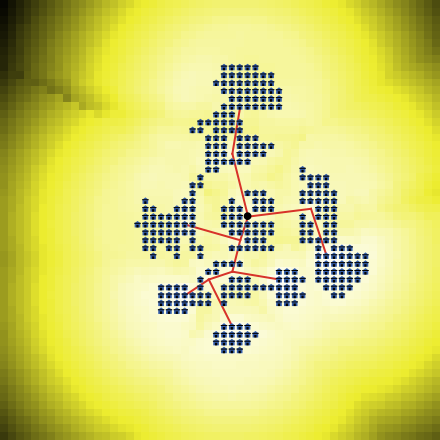
\includegraphics[width=0.55\textwidth,height=0.3\textheight]{figuresslides/intro_RBD_lattice.png}
	
	\footnotesize
\textit{Hybrid urban morphogenesis \cite{raimbault2014hybrid}}
	

	\end{column}
	\vrule{}
	\begin{column}{0.5\textwidth}
	
	\begin{center}
	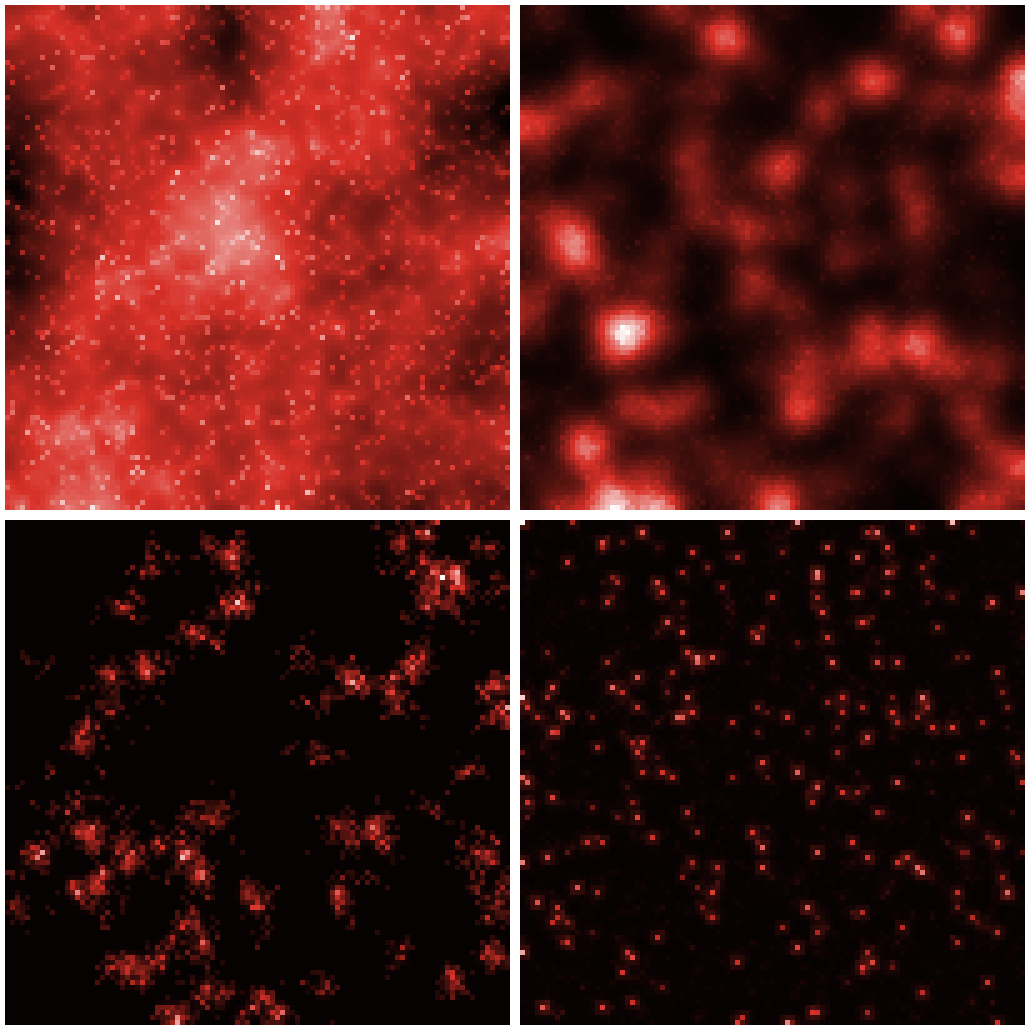
\includegraphics[width=0.5\textwidth]{figuresslides/density_Fig2}
	\end{center}
	
	\tiny
	
	\medskip
	
Raimbault, J. (2018). Calibration of a density-based model of urban morphogenesis. PloS one, 13(9), e0203516.

\nocite{raimbault2018calibration}

\smallskip

Raimbault, J. (2019). An urban morphogenesis model capturing interactions between networks and territories. In The Mathematics of Urban Morphology (pp. 383-409). Birkhäuser, Cham.

\nocite{raimbault2019urban}
	

	\end{column}

\end{columns}

}


\sframe{Urban Systems and Artificial Life}{

\begin{center}
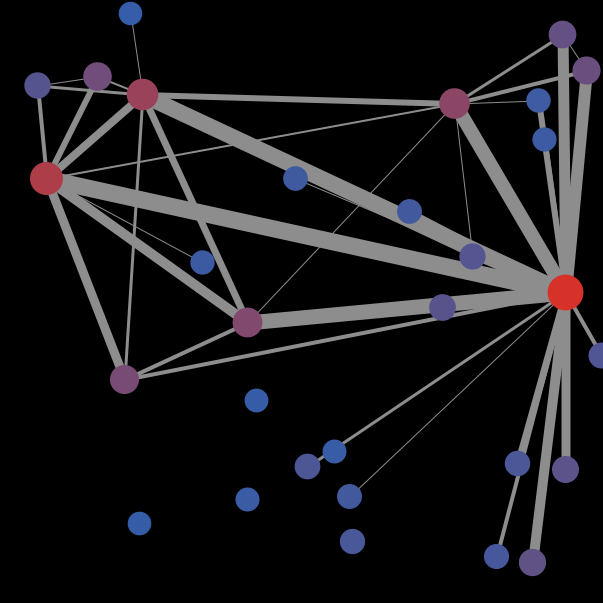
\includegraphics[height=0.47\textheight]{figuresslides/macrocoevol_example_virtual_0_tf.png}
\end{center}

	\footnotesize
	\textit{Cities-network co-evolution model explored on synthetic systems of cities} \cite{raimbault2019modeling}

	\medskip
	\hrule
	\medskip

	Model studied by~\cite{tero2010rules} : exploration and reinforcement by a slime mould searching for ressources

\bigskip

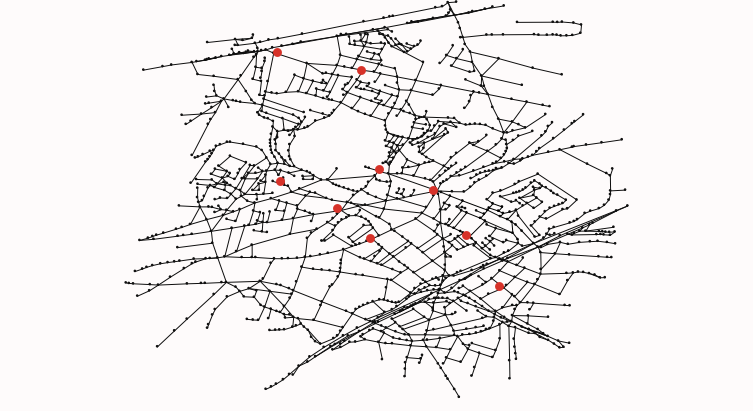
\includegraphics[width=0.32\textwidth]{figuresslides/slimemould_tick1}
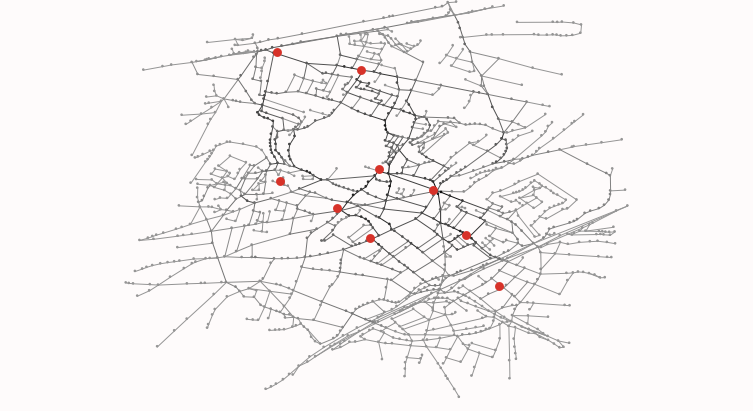
\includegraphics[width=0.32\textwidth]{figuresslides/slimemould_tick20}\\
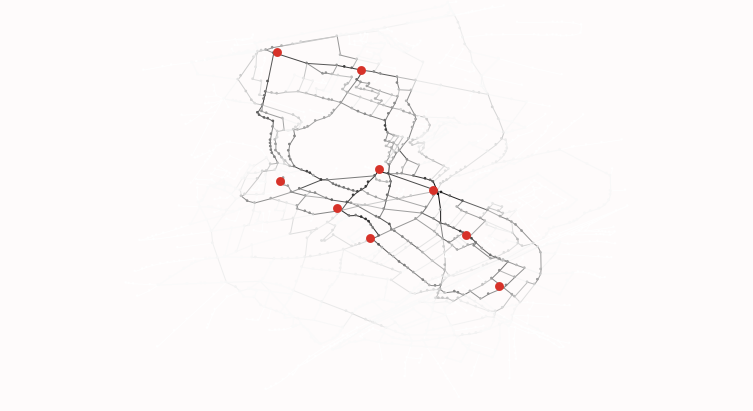
\includegraphics[width=0.32\textwidth]{figuresslides/slimemould_tick101}
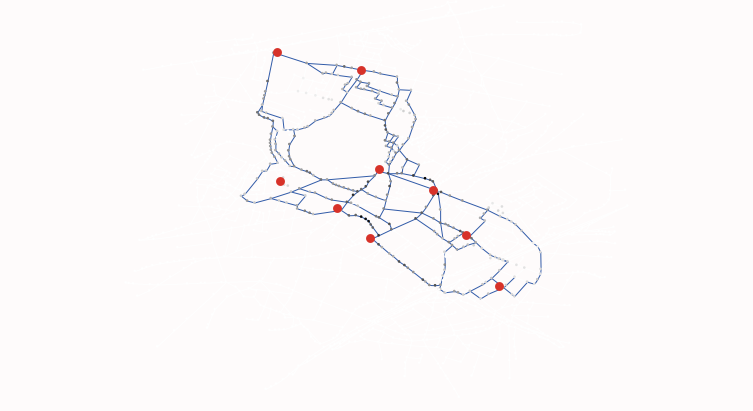
\includegraphics[width=0.32\textwidth]{figuresslides/slimemould_reseauFinal}\\
	

}





\sframe{Urban form from the bottom up}{

%systematic comparison of simple processual generators
%	\item introduction of morphological indicators
%	\item calibration on sampled layouts from OpenStreetMap

$\rightarrow$ emergence of the urban form from local processes

$\rightarrow$ 


\bigskip

\textbf{Research objective: } 

}






\sframe{Generating building layouts}{

Complementary heuristics:

\medskip

\begin{itemize}
	\item random building blocks (modern urbanism)
	\item random population kernels (preferential attachment)
	\item percolation of roads through a compact urban core (transportation flows)
\end{itemize}

}


\sframe{Quantifying urban form}{

% Simple descriptive indicators considered are (i) the total building density $A = \frac{1}{N}\cdot \sum_i s_i$; (ii) the number of buildings given by the number of connected components of $B$; (iii) the average building area, i.e. the average size of $B$ connected components; (iv) Moran index capturing spatial autocorrelation (see \cite{raimbault2018calibration} for its definition in a similar setting), with a simple inverse distance weight function; (v) average distance between non-empty points (which also captures a level of concentration).
% We also use indicators computed with the underlying networks: the average detour computed in the free space network $\bar{B}$, computed by randomly sampling 50 pairs of points in a connected component of $\bar{B}$ and computing the ratio between the network distance and the euclidian distance $d_{\bar{B}}/d_E$. This measures captures in a way the sinuosity of streets from a mobility viewpoint. We also consider the average size of open connected areas as the average size of the connected components of $\bar{B}$.
% steps for dilation + steps for erosion


Urban form indicators for building layouts:

\medskip

\begin{itemize}
	\item density, number of buildings, average area
	\item Moran index and average distance on rasterized representation
	\item average detour in the free space
	\item mathematical morphology indicators (steps for erosion and dilation) \cite{serra1994morphological}
\end{itemize}


}


\sframe{Generators}{

\textit{Examples for each generator}

\medskip

\begin{center}
	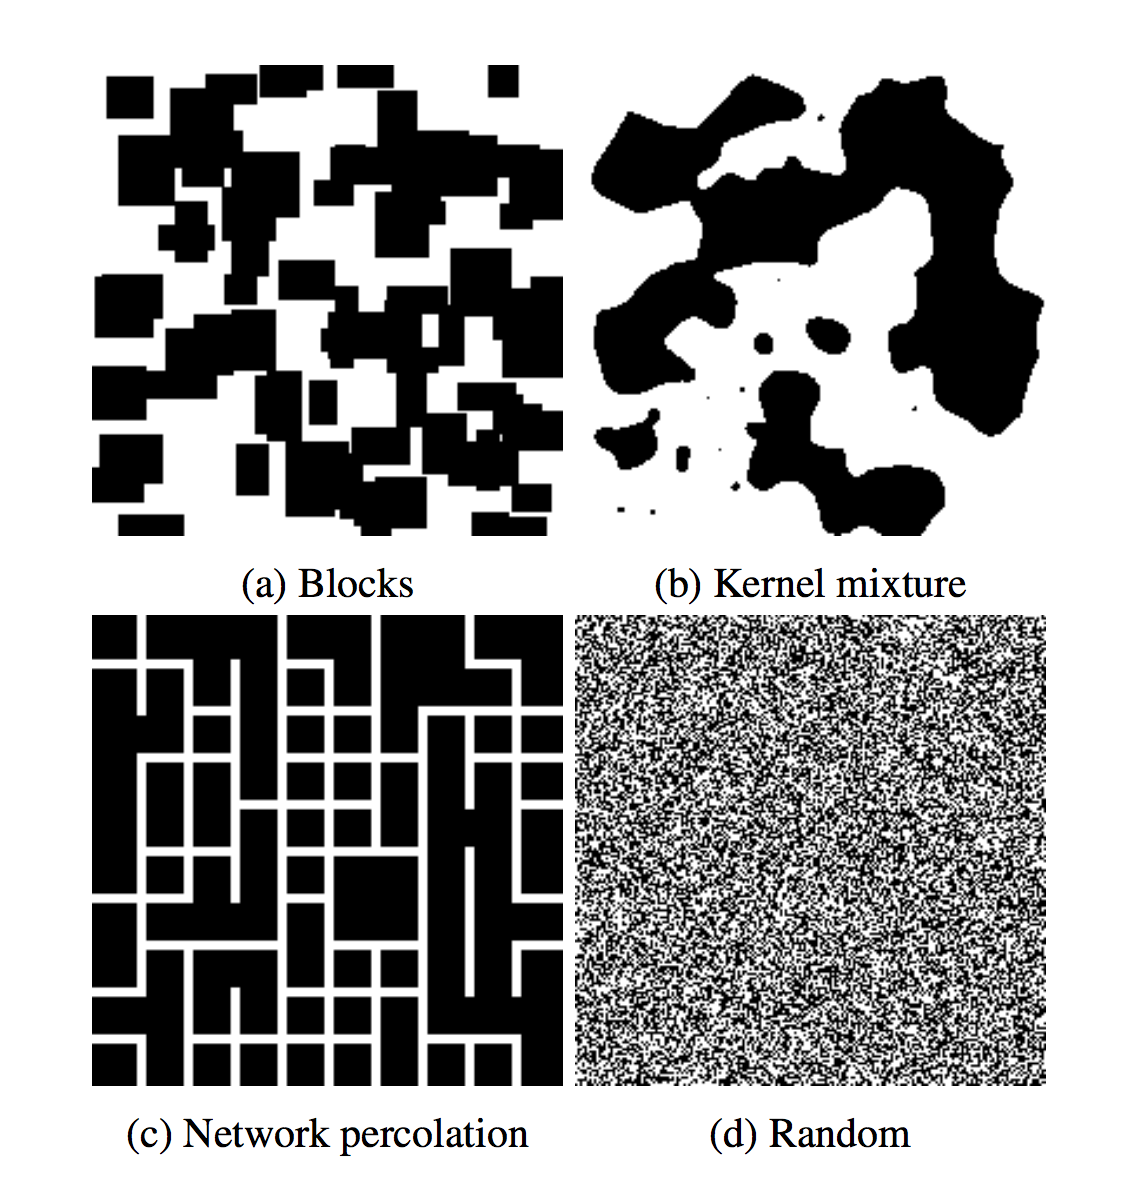
\includegraphics[height=0.85\textheight]{figuresslides/spatialsens_examplegenerators.png}
\end{center}


}

\sframe{Real configurations}{

\textit{Sampled districts from OpenStreetMap}

%\medskip

\begin{center}
	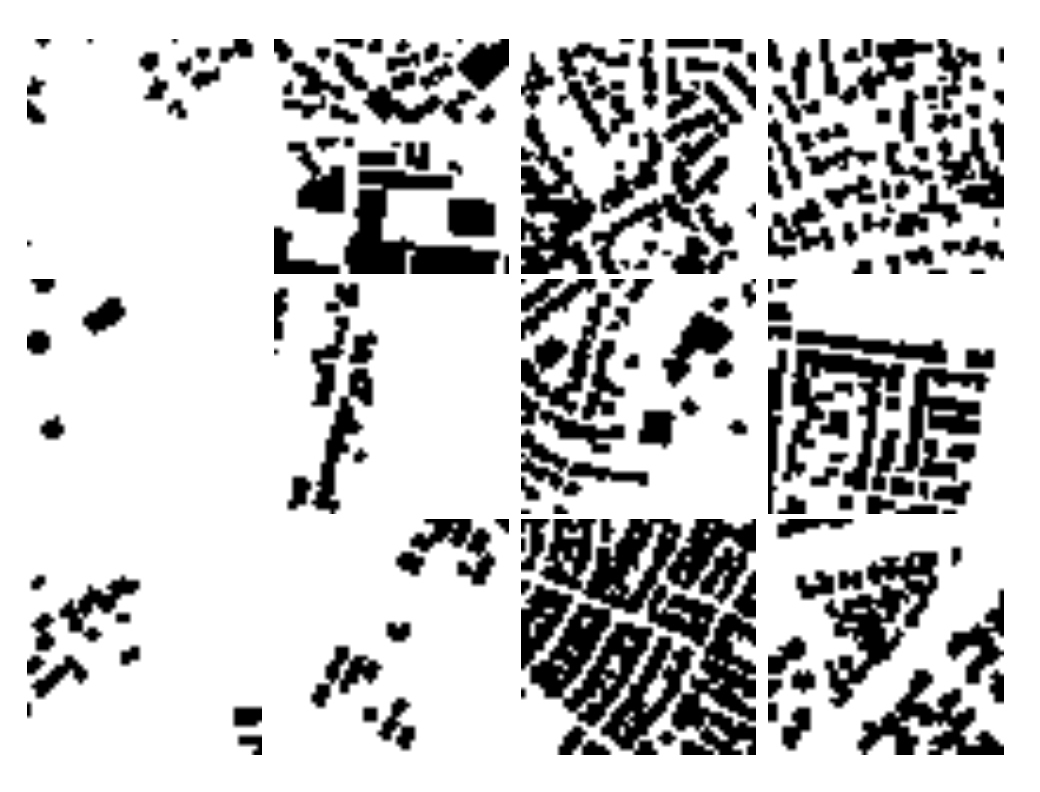
\includegraphics[height=0.85\textheight]{figuresslides/spatialsens_exampleosm.png}
\end{center}

}


\sframe{Classification of urban forms}{

\begin{center}
   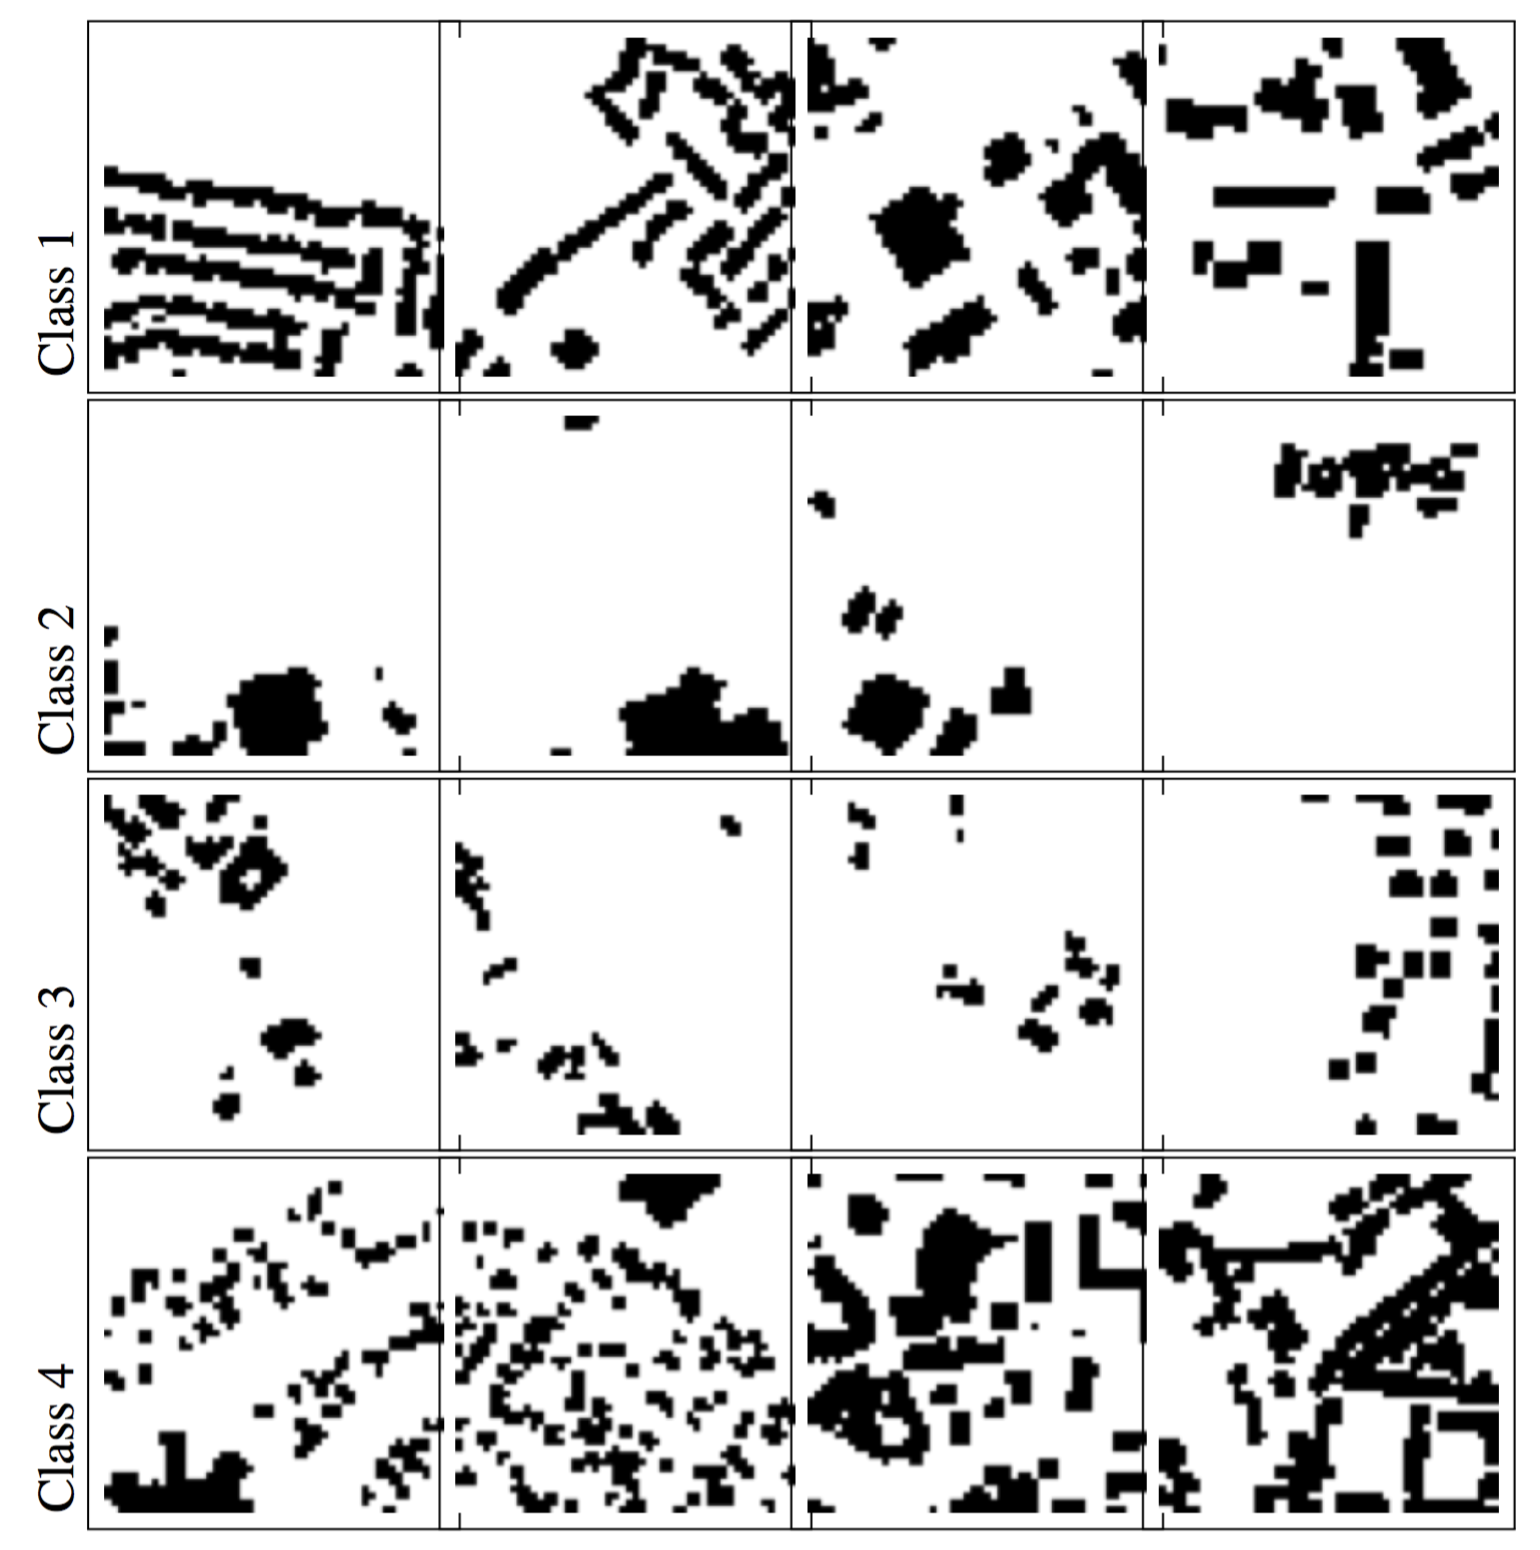
\includegraphics[height=0.9\textheight]{figuresslides/spatialsens_osm_classification.png}
\end{center}

}



\sframe{Model calibration tool}{


OpenMOLE software \url{https://next.openmole.org/}

\centering

\smallskip


\includegraphics[height=0.35\textheight]{figuresslides/openmole.png}

\smallskip

\raggedright\justify

\footnotesize \textit{OpenMOLE: (i) embed any model as a black box; (ii) transparent access to main High Performance Computing environments; (iii) model exploration and calibration methods.}

}




\sframe{Calibrated forms}{

\centering

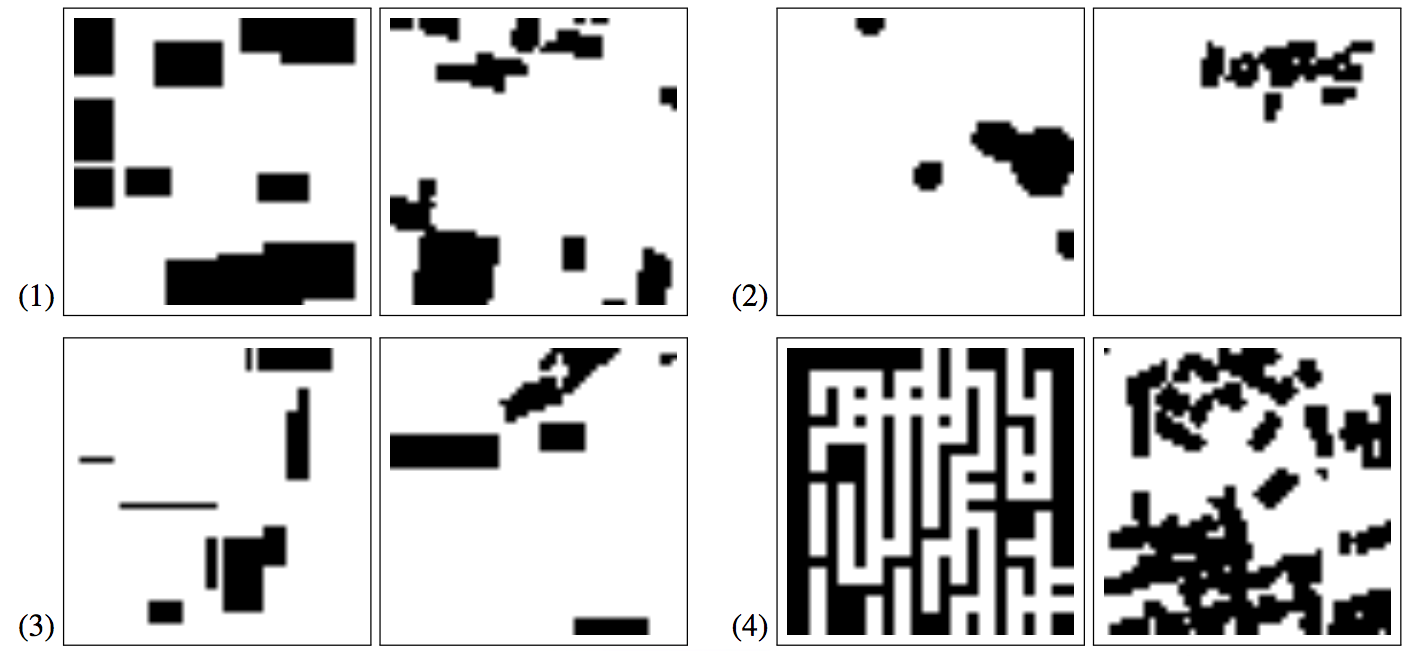
\includegraphics[width=\textwidth]{figuresslides/spatialsens_calib.png}

}


\sframe{Point cloud}{

\begin{center}
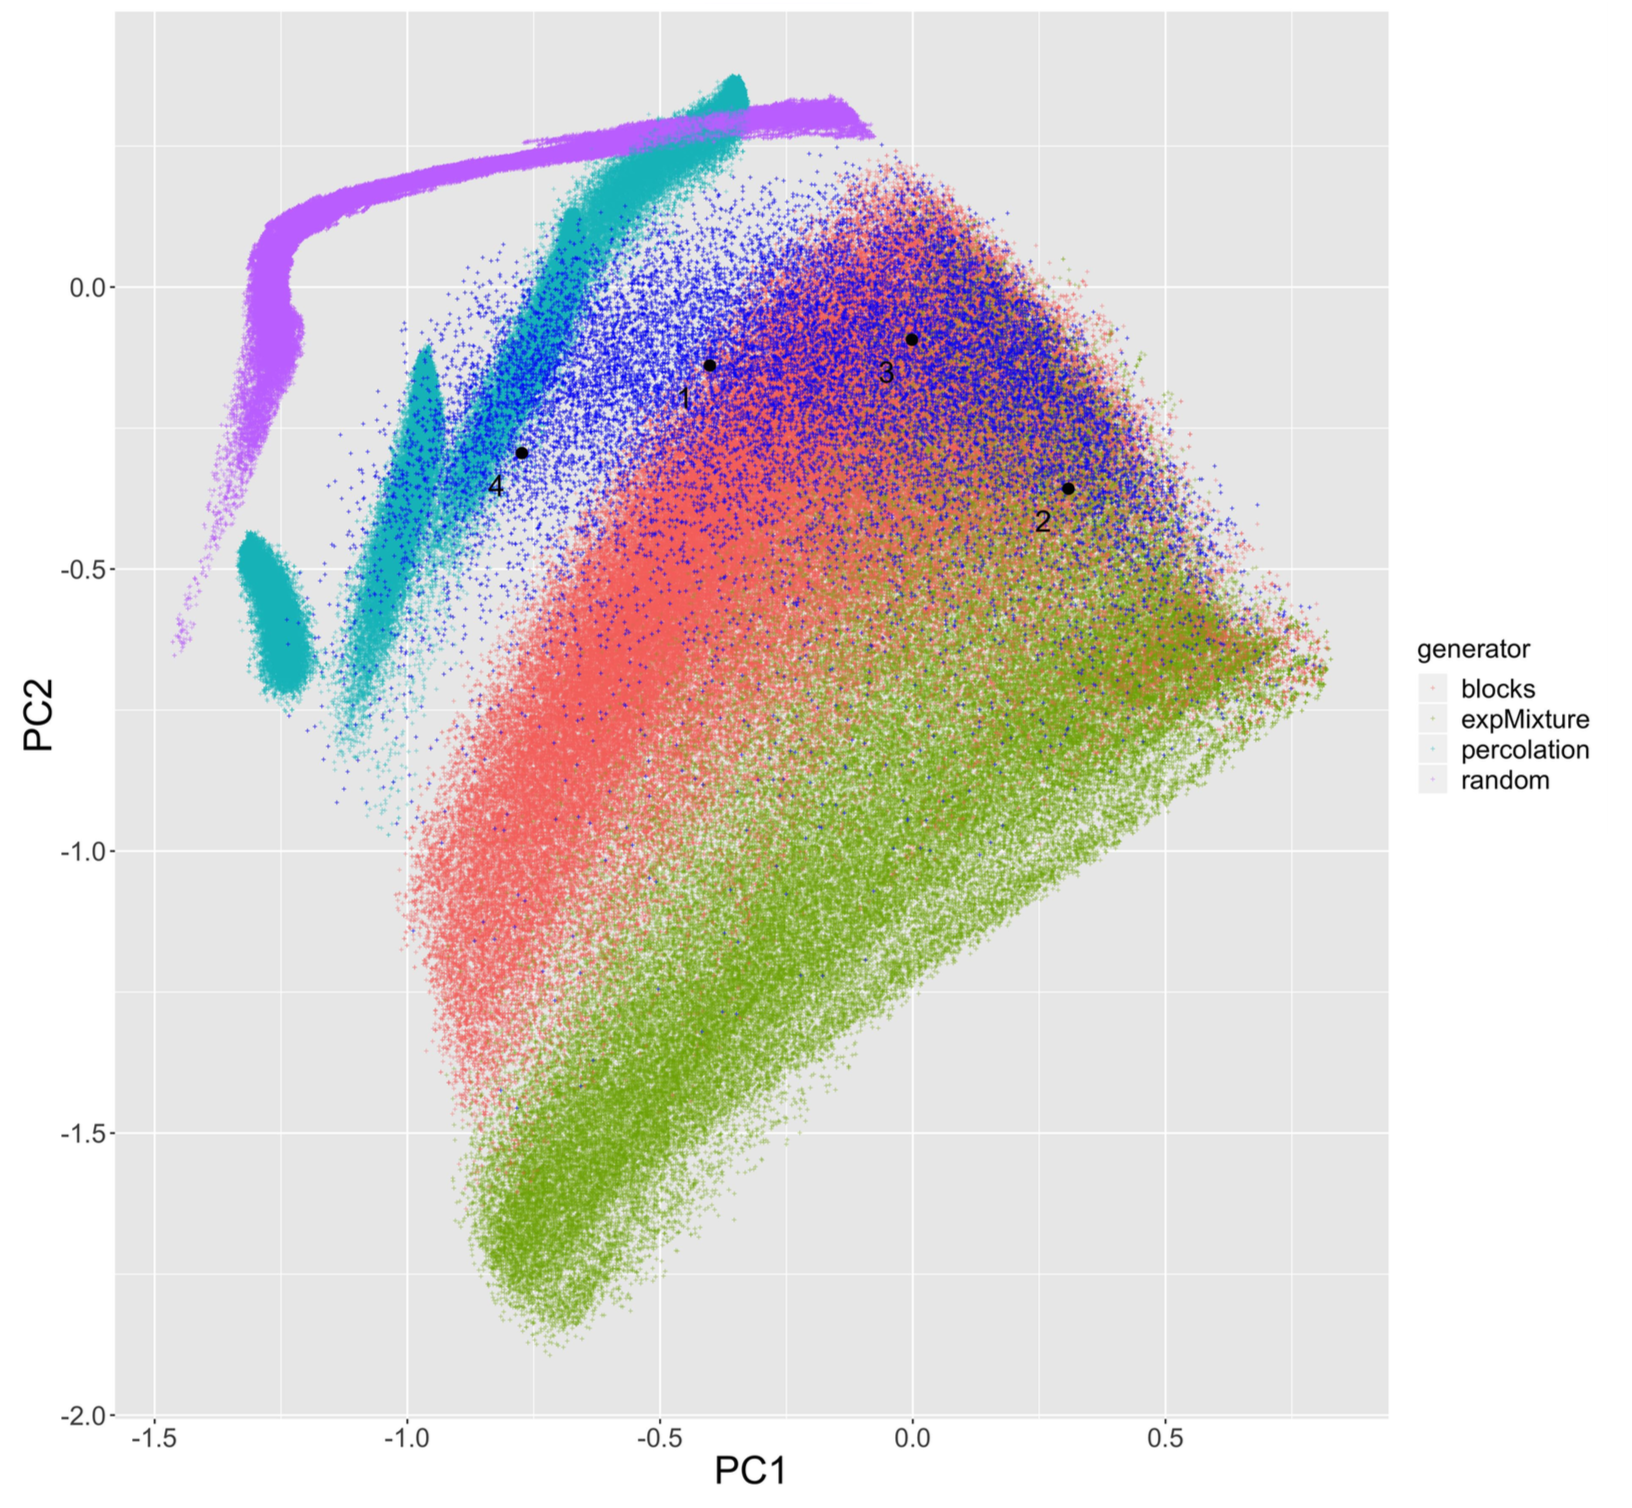
\includegraphics[height=0.9\textheight]{figuresslides/spatialsens_points.png}
\end{center}

}


\sframe{Calibration}{

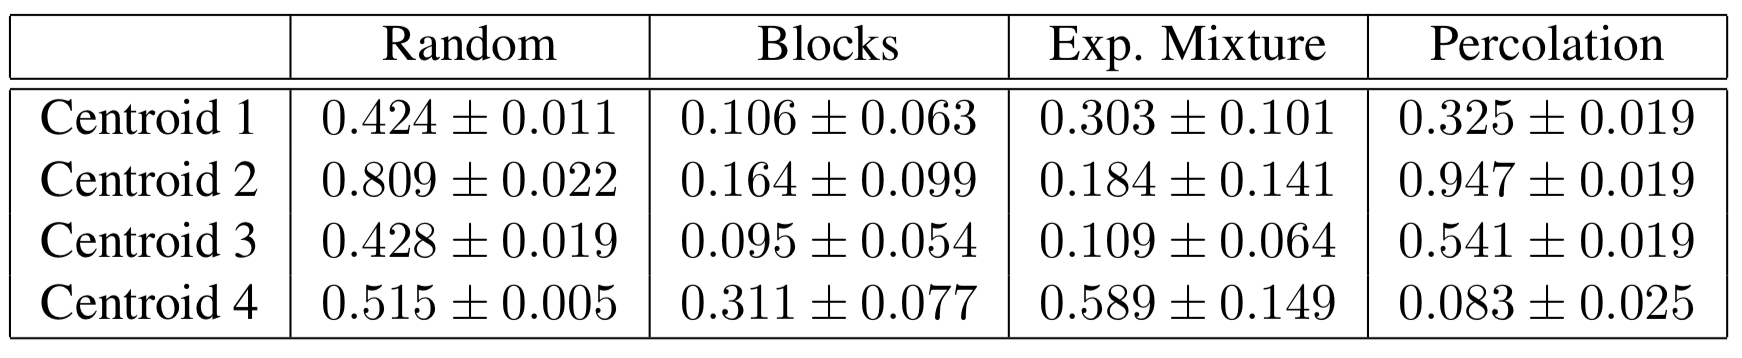
\includegraphics[width=\textwidth]{figuresslides/spatialsens_distanceclasses.png}

\medskip

\textit{Why not use calibration heuristics? Open question of fitting a point cloud; issue of projecting in a reduced dimension space}

}


\sframe{Discussion}{

%Our approach provides a first step towards systematic modeling of generative processes of urban form at large scales. Some direct limitations could be tackled in a short term. Testing slightly different processes and heuristics in generator may be a way to cover the part of the real point cloud which is missed by our generators. As it seems correspond to complicated urban centers, it may be however complicated without more elaborated models. Also, we did not use minimization algorithms to calibrate the generators, and the and a further step would consist in checking the robustness of our result using such optimization heuristics (genetic algorithms for example), but also diversity algorithms such as pattern space exploration proposed by \cite{10.1371/journal.pone.0138212}, to ensure the effective feasible space of each generator. 
%This work can also be extended in several ways. First of all, we focused on the built environment but neglected transportation infrastructures, whereas spatial network morphogenesis models have been proposed for example by \cite{courtat2011mathematics} or \cite{raimbault2018multi} in a multi-modeling approach.
%Taking into account multiple dimensions of the urban system is an important extension and hybrid models such as co-evolution models \citep{raimbault2014hybrid} should be investigated.
%\added{Our approach can also be a preliminary step towards the study of urban sustainability issues, for example the relations between urban form and energy consumption }\citep{le2015forme}.\added{ Extending the generators with the third dimension, i.e. taking into account building heights as done by }\cite{brasebin2017apports}\added{, could also be an important component for the study of local energy efficiency.}
%Furthermore, we tested the complementarity of generators only in a static way. Adaptive and dynamic generators, combining processes of different nature within the same model with an endogenous switching or combination, would be an important direction to better understand urban morphogenesis.
%In the same context, the generators compared here had all the same number of parameters, but richer generators implying different numbers would require the use of information criterions to avoid overfitting, which, however, remains an unsolved issue for such generative simulation models \citep{piou2009proposing}.
%Finally, as extensively reviewed above, the way to quantify urban form strongly depends on the scale considered. A more integrative understanding of it would require multi-scale approaches able to relate these different definition and measures within a single multi-scalar framework.




}


\sframe{Conclusion}{

\justify

$\rightarrow$

\medskip

\textit{Code and results at } \url{https://github.com/openmole/spatialdata}

 

}





%%%%%%%%%%%%%%%%%%%%%
\begin{frame}[allowframebreaks]
\frametitle{References}
\bibliographystyle{apalike}
\bibliography{biblio}
\end{frame}
%%%%%%%%%%%%%%%%%%%%%%%%%%%%






\end{document}


